\documentclass[12pt]{article}

\usepackage[margin=2cm]{geometry}
\usepackage[T2A]{fontenc}
\usepackage[utf8]{inputenc}
\usepackage[russian]{babel}
\usepackage{multicol}
\usepackage{graphics}
\usepackage{rotating}
\usepackage{float}

\setlength{\parindent}{0em}
\setlength{\parskip}{1em}

\usepackage{amsmath, amsfonts, amssymb, amsthm, mathtools}
\usepackage{icomma}

\title{Отчет о выполнении лабораторной работы \\ Определение $C_p/C_v$ по скорости звука в газе}
\author{Лепарский Роман}
\date{\today}

\begin{document}

\maketitle

\newpage

\section{Аннотация}

\textbf{Цель работы:} 1) измерение частоты колебаний и длины волны при резонансе звуковых колебаний в газе, заполняющем трубу; 2) определение показателя адиабаты с помощью уравнения состояния идеального газа.

\section{Теоретические сведения}

Скорость распространения звуковой волны в газах зависит от показателя адиабаты $\gamma$ и вычисляется по формуле:
\begin{equation} \label{eq:sound-speed}
	c=\sqrt{\gamma \frac{RT}{\mu}}
\end{equation}
Отсюда:
\begin{equation} \label{eq:gamma}
	\gamma = \frac{\mu}{RT}c^2
\end{equation}
Таким образом, для определения показателя адиабаты достаточно
измерить температуру газа и скорость распространения звука

Звуковые колебания в трубе являются наложением всех отраженных волн. Однако, если в трубку укладывается целое число полуволн,
амплитуда колебаний резко повышается -- наступает резонанс.

Скорость звука c связана с его частотой $f$ и длиной волны $\lambda$ соотношением:
\begin{equation} \label{eq:c-lambda-f}
	c = \lambda f
\end{equation}

Подбор условий, при которых возникает резонанс, можно производить двояко:

\hspace{7mm} 1. При неизменной частоте f звукового генератора можно изменять длину трубы L. Для этого применяется раздвижная труба. Длина раздвижной трубы постепенно увеличивается, и наблюдается ряд последовательных резонансов. Для каждого из них имеем:
\begin{equation}
	L_{k} = (n+k)\frac{\lambda}{2}
\end{equation}
Таким образом, можно найти $\frac{\lambda}{2}$ как угловой коэффициент зависимости длинны трубы от номера резонанса.

\hspace{7mm} 2. При постоянной длине трубы можно изменять частоту звуковых колебаний, а следовательно, и длину звуковой волны $\lambda$.
Для последовательных резонансов получим:
\begin{equation} \label{eq:len}
	L = \frac{\lambda_k}{2}(n+k)
\end{equation}

Из (\ref{eq:c-lambda-f}) и (\ref{eq:len}) получим:
\begin{equation}
	f_{k+1}  = f_1 + \frac{c}{2L}k
\end{equation}
Скорость звука, деленная на $2L$, определяется, таким образом,
по угловому коэффициенту графика зависимости частоты от номера
резонанса.

\subsection*{Методика измерений}

\begin{figure}[H]
	\centering
	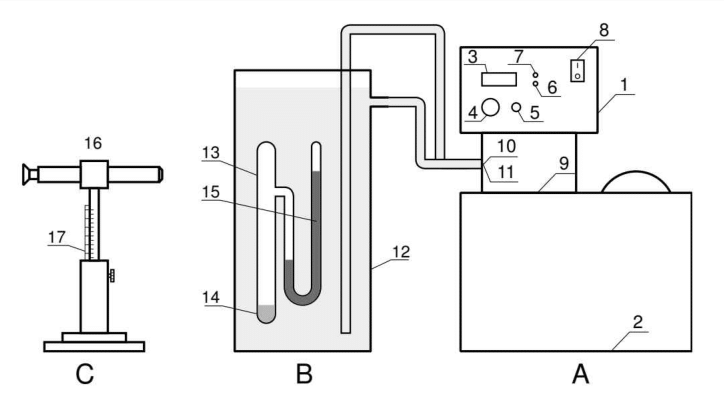
\includegraphics[scale=0.3]{stand.png}
\end{figure}

В обеих установках звуковые колебания в трубе возбуждаются телефоном Т и улавливаются микрофоном М. Они присоединены к установке через тонкие резиновые трубки. Такая связь достаточна для возбуждения и обнаружения звуковых колебаний в трубе и в то же время мало возмущает эти колебания.

Первая установка (рис. 1) содержит раздвижную трубу с миллиметровой шкалой. Через патрубок (на рисунке не показан) труба может наполняться воздухом или углекислым газом из газгольдера. На этой установке производятся измерения $\gamma$ для воздуха и для CO$_2$.


Вторая установка (рис. 2) содержит теплоизолированную трубу постоянной длины. Воздух в трубе нагревается водой из термостата. Температура газа принимается равной температуре омывающей трубу воды. На этой установке измеряется зависимость скорости звука от температуры.

\section{Приборы и материалы}

В работе используются:

\begin{itemize}
	\item Звуковой генератор;
	\item Электронный осциллограф;
	\item Микрофон;
	\item Телефон;
	\item Раздвижная труба;
	\item Теплоизолированная труба, обогреваемая водой из термостата;
	\item Баллон со сжатым углекислым газом;
	\item Газгольдер.
\end{itemize}

\section{Обработка результатов}

\subsection{Эксперимент 1}

Обработаем значения, полученные для воздуха. Погрешность измерения длины трубки $\Delta L = 0.5$мм, частоты $\Delta f = 0.05$кГц

\begin{table}[H]
	\centering
	\caption{Измерения для воздуха при различных частотах}
	\begin{tabular}{|l|l|l|l|l|}
		\hline
		& $f = 2$kHz & $f = 3$kHz & $f = 4$kHz & $f = 5$kHz \\ \hline
		N & $L$, mm    & $L$, mm    & $L$, mm    & $L$, mm    \\ \hline
		1 & 34.5       & 7.5        & 36.5       & 21.0       \\ \hline
		2 & 120.5      & 66.0       & 79.0       & 56.0       \\ \hline
		3 & 208.0      & 123.0      & 121.5      & 90.5       \\ \hline
		4 &            & 180.5      & 164.5      & 125.0      \\ \hline
		5 &            &            & 207.0      & 160.0      \\ \hline
		6 &            &            &            & 194.5      \\ \hline
	\end{tabular}
\end{table}

\begin{minipage}[t]{.49\textwidth}
	\vspace{0pt}
	\centering
		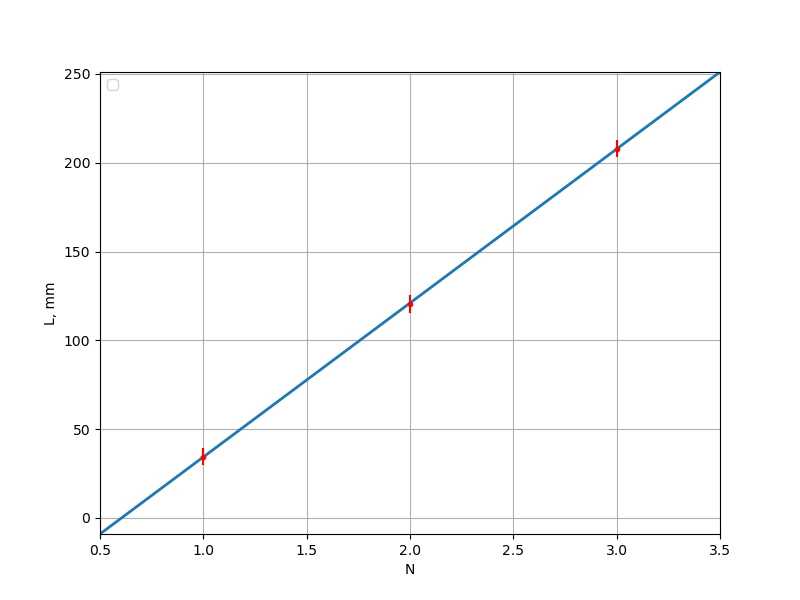
\includegraphics[scale = 0.45]{O2_2.png}
		\small{$f = 2$kHz, $\lambda/2 = 86,7\pm0.3$mm}
\end{minipage}
\begin{minipage}[t]{.49\textwidth}
	\vspace{0pt}
	\centering
	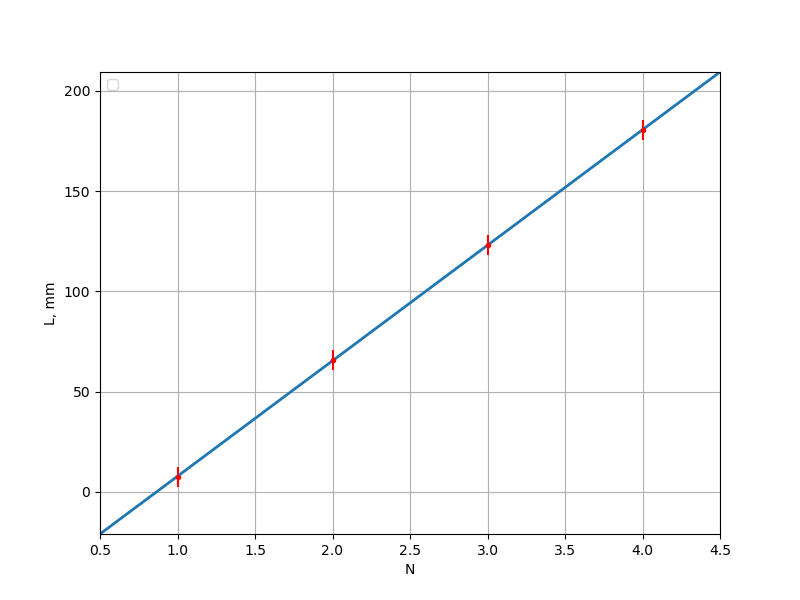
\includegraphics[scale = 0.45]{O2_3.png}
	\small{$f = 3$kHz, $\lambda/2 = 57.60\pm0.15$mm}
\end{minipage}

\begin{minipage}[t]{.49\textwidth}
	\vspace{0pt}
	\centering
	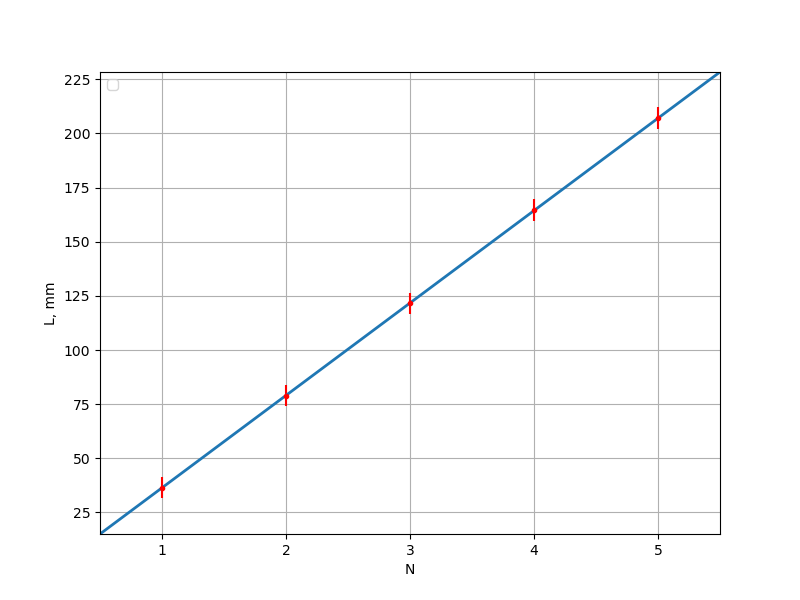
\includegraphics[scale = 0.45]{O2_4.png}
	\small{$f = 4$kHz, $\lambda/2 = 42.65\pm0.03$mm}
\end{minipage}
\begin{minipage}[t]{.49\textwidth}
	\vspace{0mm}
	\centering
	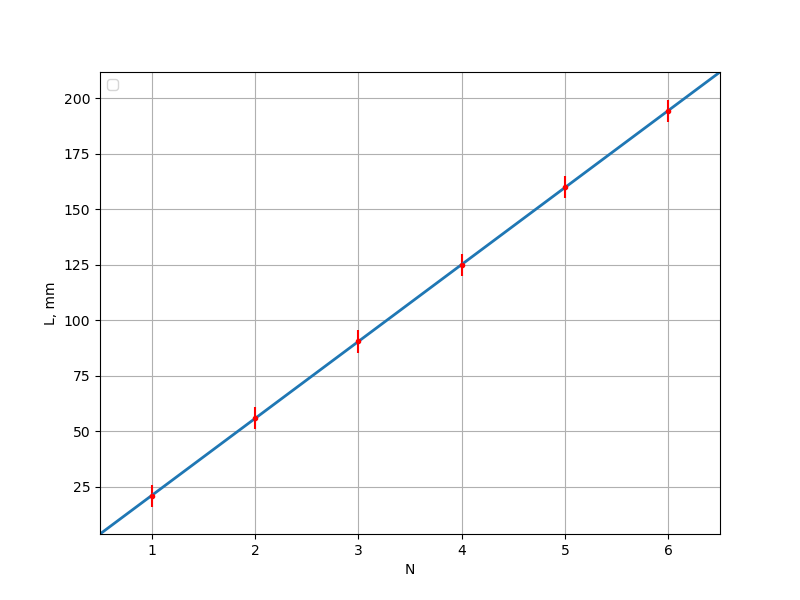
\includegraphics[scale = 0.45]{O2_5.png}
	\small{$f = 5$kHz, $\lambda/2 = 34.69\pm0.03$mm}
\end{minipage}

Скорость звука рассчитаем по формуле (\ref{eq:c-lambda-f}), а погрешность следующим образом:
\begin{equation*}
	\sigma_c^2 = (f \sigma_{\lambda})^2 + (\lambda \sigma_{f})^2
\end{equation*}

\begin{table}[H]
	\centering
	\begin{tabular}{|l|l|l|}
		\hline
		$f$, kHz & $c$, m/s & $\sigma_c$, m/s \\ \hline
		2        & 347      & 9               \\ \hline
		3        & 346      & 6               \\ \hline
		4        & 341      & 4               \\ \hline
		5        & 347      & 3               \\ \hline
	\end{tabular}
\end{table}

Итого $c = 345 \pm 6$m/s. Комнатную температуру примем 295К, и посчитаем коэффициент адиабаты.
\begin{equation*}
	\gamma = \frac{\mu}{RT}c^2 = 1.41
\end{equation*}
\begin{equation*}
\sigma_\gamma = \frac{2\mu}{RT}c\cdot\sigma_c = 0.04
\end{equation*}

Приступим к обработке измерений для CO$_2$
\begin{table}[H]
	\centering
	\caption{Измерения для CO$_2$ при различных частотах}
	\begin{tabular}{|l|l|l|l|l|}
		\hline
		& $f = 2$kHz & $f = 2.5$kHz & $f = 3$kHz & $f = 3.5$kHz \\ \hline
		N & $L$, mm    & $L$, mm      & $L$, mm    & $L$, mm      \\ \hline
		1 & 44.5       & 32.5         & 18.0       & 18.0         \\ \hline
		2 & 114.0      & 90.0         & 64.0       & 57.5         \\ \hline
		3 & 184.5      & 146.5        & 111.5      & 96.5         \\ \hline
		4 &            & 202.0        & 156.5      & 136.5        \\ \hline
		5 &            &              & 204.5      & 175.5        \\ \hline
		6 &            &              &            & 213.5        \\ \hline
	\end{tabular}
\end{table}

\begin{minipage}[t]{.49\textwidth}
	\vspace{0pt}
	\centering
	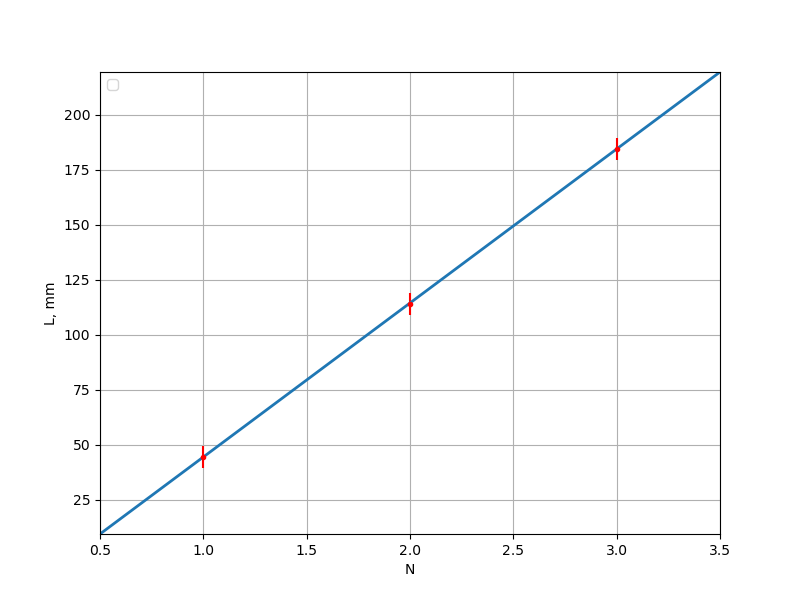
\includegraphics[scale = 0.45]{CO2_2.png}
	\small{$f = 2$kHz, $\lambda/2 = 70,00\pm0.17$mm}
\end{minipage}
\begin{minipage}[t]{.49\textwidth}
	\vspace{0pt}
	\centering
	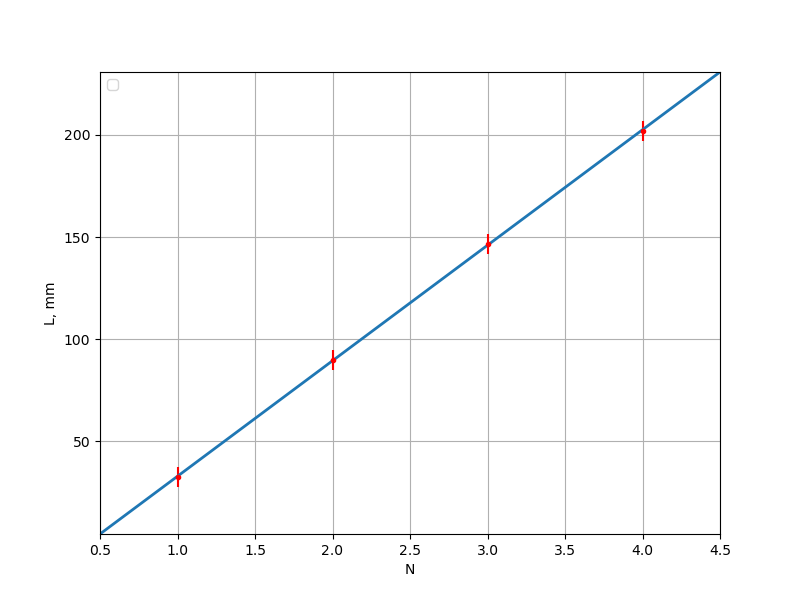
\includegraphics[scale = 0.45]{CO2_3.png}
	\small{$f = 2.5$kHz, $\lambda/2 = 56.5\pm0.2$mm}
\end{minipage}

\begin{minipage}[t]{.49\textwidth}
	\vspace{0pt}
	\centering
	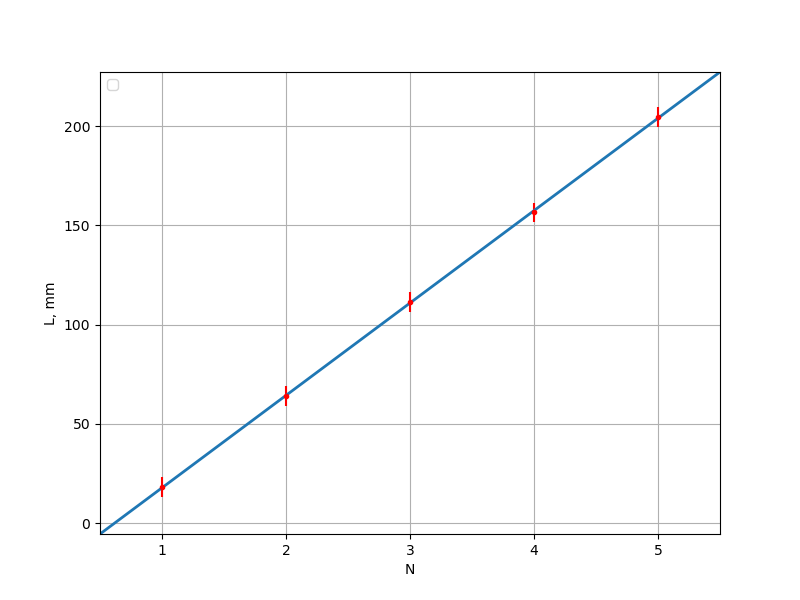
\includegraphics[scale = 0.45]{CO2_4.png}
	\small{$f = 3$kHz, $\lambda/2 = 46.55\pm0.18$mm}
\end{minipage}
\begin{minipage}[t]{.49\textwidth}
	\vspace{0pt}
	\centering
	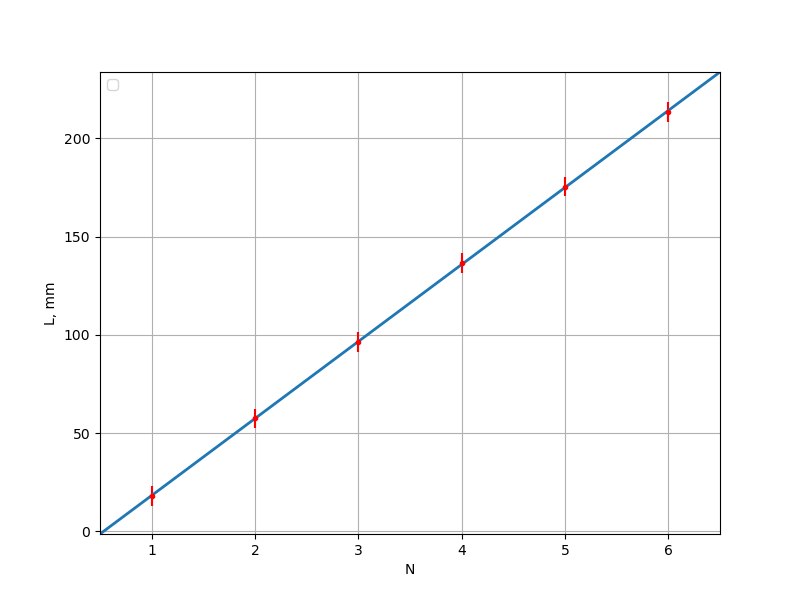
\includegraphics[scale = 0.45]{CO2_5.png}
	\small{$f = 3.5$kHz, $\lambda/2 = 39.19\pm0.11$mm}
\end{minipage}

Аналогично рассчитаем скорость звука

\begin{table}[H]
	\centering
	\begin{tabular}{|l|l|l|}
		\hline
		$f$, kHz & $c$, m/s & $\sigma_c$, m/s \\ \hline
		2        & 280      & 7               \\ \hline
		2.5        & 282      & 6               \\ \hline
		3        & 279      & 5               \\ \hline
		3.5        & 274      & 4               \\ \hline
	\end{tabular}
\end{table}

Усреднив значения, получим $c = 278\pm 6$m/s, $\gamma = 1.39\pm 0.06$

\subsection{Эксперимент 2}

Длинна трубки $L_0 = 700\pm1$mm. Внесем результаты эксперимента в таблицу.

\begin{table}[H]
	\centering
	\caption{Зависимость частоты от порядка резонанса}
	\begin{tabular}{|l|l|l|l|}
		\hline
		& t = 25$^\circ C$ & t = 35$^\circ C$ & t = 45$^\circ C$ \\ \hline
		N & f, Hz            & f, Hz            & f, Hz            \\ \hline
		1 & 742.5            & 508.5            & 772.5            \\ \hline
		2 & 997.5            & 749.5            & 1027.5           \\ \hline
		3 & 1241.5           & 994.0            & 1274.0           \\ \hline
		4 & 1480.0           & 1264.0           & 1530.0           \\ \hline
		5 & 1731.5           & 1510.5           & 1782.5           \\ \hline
		6 & 1959.5           & 1756.0           & 2045.5           \\ \hline
	\end{tabular}
\end{table}

\begin{figure}[H]
	\centering
	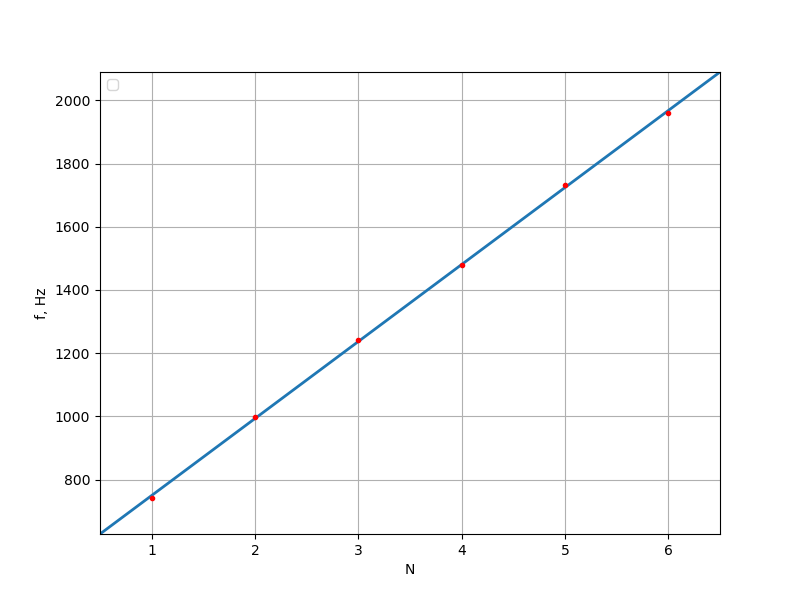
\includegraphics[scale = 0.5]{T25.png}
	\caption{Измерения при t = 25$^\circ C$, $k = 244 \pm 2$Hz}
\end{figure}

\begin{figure}[H]
	\centering
	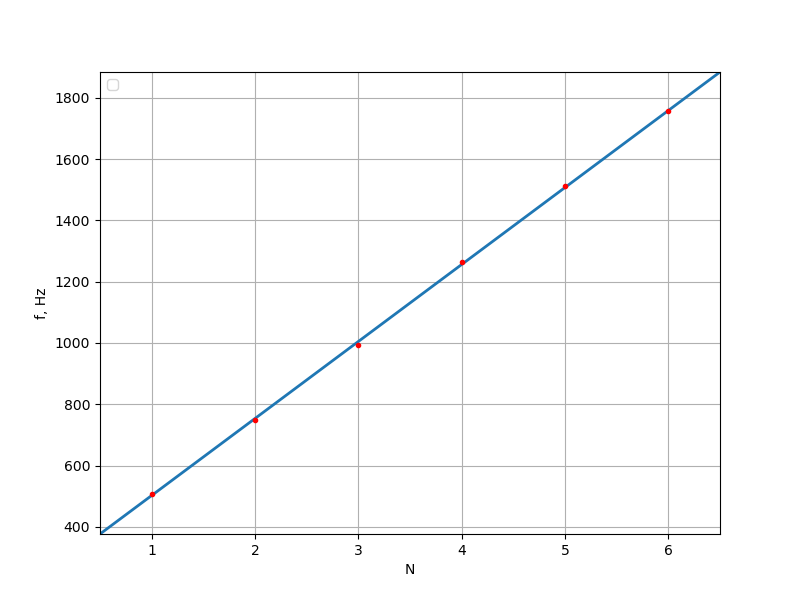
\includegraphics[scale = 0.5]{T35.png}
	\caption{Измерения при t = 35$^\circ C$, $k = 251 \pm 2$Hz}
\end{figure}

\begin{figure}[H]
	\centering
	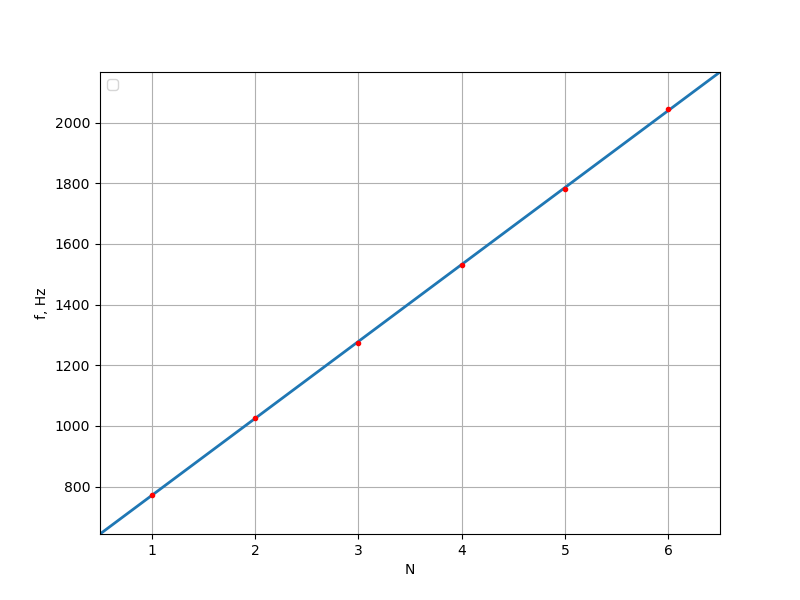
\includegraphics[scale = 0.5]{T45.png}
	\caption{Измерения при t = 45$^\circ C$, $k = 254 \pm 1$Hz}
\end{figure}

Посчитаем скорость звука по формуле $c = k\cdot 2L_0$, а та же показатель адиабаты и погрешности.

\begin{table}[H]
	\centering
	\begin{tabular}{|l|l|l|l|l|}
		\hline
		t, $^\circ C$ & $c$, m/s & $\sigma_c$, m/s & $\gamma$ & $\sigma_\gamma$ \\ \hline
		25            & 341      & 3               & 1.36     & 0.03            \\ \hline
		35            & 351      & 3               & 1.40     & 0.03            \\ \hline
		45            & 355      & 2               & 1.38     & 0.03            \\ \hline
	\end{tabular}
\end{table}

Усредняя значения получим $\gamma = 1.38 \pm 0.03$

\section{Вывод}

Как итог проведения двух экспериментов были получены скорости звука в воздухе ($345 \pm 6$m/s) и в CO$_2$ ($278\pm 6$m/s), а так же вычислен показатель адиабаты для CO$_2$ $\gamma = 1.38 \pm 0.03$ и для воздуха $\gamma = 1.41 \pm 0.04$. Из работы можно видеть, что оба метода одинаково точно оценивают эти величины и получившиеся значения находятся ,близко к табличным: для воздуха $c = 335$m/s, $\gamma = 1.40$, для CO$_2$ $c = 260$m/s, $\gamma = 1.30$. Расхождение данных полученных для CO$_2$ может быть связано с тем, что в трубе находилась примесь воздуха с предыдущего эксперимента

\end{document}